%\documentclass[8pt, handout]{beamer}
%\usepackage{pgfpages} 								%Для распечатки
%\pgfpagesuselayout{2 on 1}[a4paper,border shrink=10mm]

\documentclass[8pt]{beamer}

\usepackage[english,russian]{babel}
\usepackage[utf8]{inputenc}
\usepackage{mflogo}
\usepackage{amsmath,amsfonts,amssymb}
\usepackage{graphicx}
\usepackage{xcolor}
\usepackage{transparent}



\beamertemplatenavigationsymbolsempty

\usetheme{EastLansing}
\setbeamercovered{transparent}


\title[Действительные числа, функции, последовательности]{Математический анализ\\ Тема 1: Действительные числа, функции, последовательности}
\author[Выборный Е. В.]{Выборный Евгений Викторович\\ email: evybornyi@hse.ru}
\date{Москва 2015} 


\makeatletter
\setbeamertemplate{footline}{
    \leavevmode%
    \hbox{%
    \begin{beamercolorbox}[wd=.25\paperwidth, ht=2.5ex, dp=1ex, center]{author in head/foot}%
        \usebeamerfont{author in head/foot}%
        \insertshortauthor
    \end{beamercolorbox}%
    \begin{beamercolorbox}[wd=.5\paperwidth,ht=2.5ex,dp=1ex,center]{title in head/foot}%
        \usebeamerfont{title in head/foot}\insertshorttitle
    \end{beamercolorbox}%
    \begin{beamercolorbox}[wd=.25\paperwidth,ht=2.5ex,dp=1ex,right]{date in head/foot}%
        \usebeamerfont{date in head/foot}\insertshortdate{}\hspace*{2em}
        \insertframenumber{} / \inserttotalframenumber\hspace*{2ex}
    \end{beamercolorbox}}%
    \vskip0pt%
}
\makeatother

\makeatletter
\setbeamertemplate{title page}
{
\centering
 \usebeamerfont{author}\insertauthor
 \vfill
 \begin{beamercolorbox}[rounded=true,shadow=true,sep=8pt,center]{title}
  \usebeamerfont{title}\inserttitle
 \end{beamercolorbox}
\vfill
\centering
\insertdate\par
 \vskip0.2em
}
\makeatother

\begin{document}
%\parindent=1.5em %красная строка

\begin{frame}
\titlepage
\end{frame}

\begin{frame}{Базовые обозначения}
\begin{block}{Обозначения}
Мы будем использовать следующие стандартные математические обозначения:
\begin{itemize}
\item $\Rightarrow$ --- ``следует'';
\item $\Leftrightarrow$ --- ``равносильно''  или ``справедливо тогда, и только тогда, когда'';
\item $\forall$ --- ``для любого'';
\item $\exists$ --- ``существует'';
\item $\in$ --- ``принадлежит'' или ``является элементом множества'';
\pause
\item $\mathbb{N}$ --- множество всех {\bf натуральных} чисел, то есть 
$$\mathbb{N}=\{ 1, 2, 3, \ldots \};$$
\item $\mathbb{Z}$ --- множество всех {\bf целых} чисел, то есть 
$$\mathbb{Z}=\{ 0, 1, -1, 2, -2, \ldots \}.$$
\end{itemize}
\end{block}
\vskip-1em
\pause
\begin{block}{Примеры}
\begin{itemize}
\item Если $n$ --- произвольное целое число ($n\in\mathbb{Z}$), то
$n>5 \Rightarrow n>3$, но $n>5 \nRightarrow n>10$.

\item $\forall n \in \mathbb{N}\ \exists m \in \mathbb{N} : m > n.$ (Всегда существует натуральное число, большее наперед заданного натурального числа)
\end{itemize}
\end{block}
\end{frame}

\begin{frame}{Элементы теории множеств}
\begin{uncoverenv}<1->
Множество --- совокупность объектов произвольной природы. 

Например, $M=\{ a, b, c, d \}$ --- множество из четырех элементов.
$$a\in M, \quad e\notin M.$$

Множество четных чисел: $E = \left\{ n\in \mathbb{Z} \mid \exists k\in\mathbb{Z}: n = 2k \right\}$.

Пустое множество $\emptyset$ --- множество, не содержащие ни одного элемента.
\end{uncoverenv}

\begin{block}{Определение (подмножество)}<2->
Множество $A$ является подмножеством множества $B$, пишут $A \subset B$, тогда и только тогда, когда 
любой элемент $a \in A$ принадлежит множеству $B$:
$$A\subset B\quad \Leftrightarrow\quad (a\in A \Rightarrow a\in B).$$

\begin{center}
\only<1>{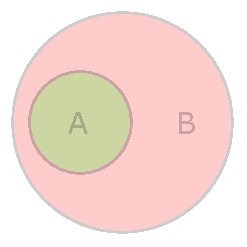
\includegraphics[scale=0.6]{subset1v0.pdf}}
\only<2>{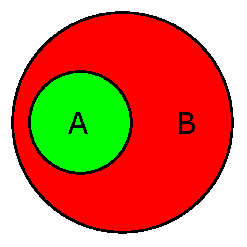
\includegraphics[scale=0.6]{subset1.pdf}}
\end{center}
\vskip-1em
\end{block}
\end{frame}

\begin{frame}{Натуральный ряд $\mathbb{N}$}
Для доказательства утверждений, зависящих от натурального параметра $n \in \mathbb{N}$, часто используется метод математической индукции.

\begin{block}{Метод математической индукции}
Пусть для утверждения $A(n)$, зависящего от параметра $n\in\mathbb{N}$, верно, что:
\begin{itemize}
\item $A(n)$ верно при $n=1$;
\item для любого $n\in\mathbb{N}$ из того, что справедливо $A(n)$, следует, что справедливо $A(n+1)$.
\end{itemize}
Тогда $A(n)$ справедливо для любых $n\in\mathbb{N}$.
\end{block}

\pause
\begin{block}{Пример}
$$A(n): \quad 1+2+3+\cdots+n = \frac{n(n+1)}{2}.$$
\end{block}
\pause
\vskip-1em
\begin{block}{Доказательство}
{\bf База индукции} ($n=1$):
$$1=\frac{1(1+1)}{2}.$$
{\bf Шаг индукции.} Используем $A(n)$ для доказательства $A(n+1)$:
$${\color{red} 1+2+3+\cdots+n }+(n+1) = {\color{red} \frac{n(n+1)}{2}}+(n+1)=\frac{(n+1)(n+2)}{2}.$$
\end{block}
\end{frame}

\begin{frame}{Рациональные числа $\mathbb{Q}$}

\begin{block}{Определение. Рациональное число}
Рациональное число --- это число, представляемое обыкновенной дробью $\displaystyle \frac{m}{n}$, где числитель $m$ --- целое число, а знаменатель $n$ --- натуральное число:
$$\mathbb{Q}= \left\{ \frac{m}{n} \mid m\in\mathbb{Z}, n\in\mathbb{N} \right\}.$$
При этом одно число может быть представлено различными дробями. Например:
$$\displaystyle \frac{2}{4}=\frac{1}{2},$$
$$ \frac{3}{1}=\frac{9}{3}.$$
\end{block}

Очевидно, целые числа $\mathbb{Z}$ являются частным случаем рациональных $\mathbb{Q}$:
$$\mathbb{Z} \subset \mathbb{Q},$$
так как $\forall r\in \mathbb{Z}$ имеется представление в виде дроби $r=\displaystyle \frac{r}{1} \in \mathbb{Q}$.
\end{frame}

\begin{frame}{Рациональные числа $\mathbb{Q}$}
\begin{block}{Предложение}
Число $\sqrt{2}$ (число, квадрат которого равен 2) не является рациональным.
\end{block}
\pause
\begin{block}{Доказательство}
Предположим обратное. Пусть $\displaystyle \sqrt{2}=\frac{m}{n},$
где $\displaystyle \frac{m}{n}$ --- несократимая дробь. Тогда
$$2=\frac{m^2}{n^2},$$
$$
m^2=2 n^2  \Rightarrow\ 
\text{$m^2$ делится на 2} \ \Rightarrow\ 
\text{$m$ делится на 2}.
$$
\pause
Следовательно, существует целое число $k$ такое, что $m=2 k$. Тогда
$$2=\frac{4k^2}{n^2},$$
$$
4k^2=2n^2 \ \Rightarrow\ 
n^2=2 k^2  \ \Rightarrow\
\text{$n^2$ делится на 2} \ \Rightarrow\
\text{$n$ делится на 2}.
$$
Получили, что числа $n$ и $m$ оба делятся на 2. Это противоречит тому, что $n/m$ --- несократимая дробь.
\end{block}
\end{frame}

\begin{frame}{Действительные числа $\mathbb{R}$}
Рациональных чисел недостаточно для решения простых геометрических задач таких, как нахождение длины диагонали квадрата со стороной $1$ (число $\sqrt{2}$) или длины окружности с единичным радиусом (число $2\pi$).
\vskip1em
Существует различные подходы к определению понятия вещественного (действительного) числа:
\begin{itemize}
\item Дедекиндовы сечения
$$\sqrt{2}=\left\{ q\in\mathbb{Q} \mid q^2<2 \right\}.$$
\item Теория бесконечных десятичных дробей
$$\sqrt{2}=1.414213562373095048801688724209698078569671875376\ldots$$
\item Геометрический подход --- действительные числа как точки на прямой
\begin{center}
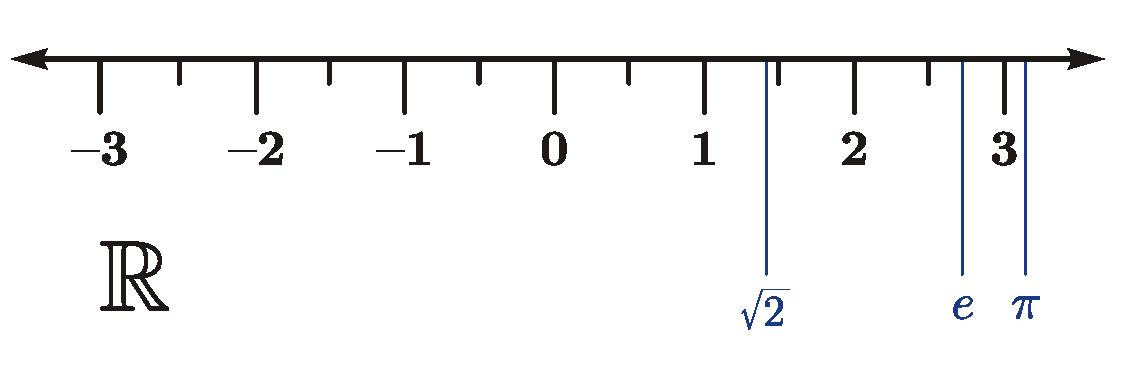
\includegraphics[scale=0.3]{pictR.pdf}
\end{center}
\end{itemize}
\pause
На множестве действительных чисел стандартным образом вводятся арифметические операции ($+$, $-$, $\times$, $/$), модуль числа, сравнения чисел ($<$, $>$, $\le$, $\ge$).

\end{frame}

\begin{frame}{Модуль действительного числа}
\begin{block}{Определение}
Модулем (абсолютной величиной) числа $x$ называют неотрицательное число $|x|$ такое, что
$$|x|=\left\{ \begin{array}{cl}
x & x\ge 0;\\
-x & x<0.
\end{array}\right.
$$
\end{block}
\vskip-1em

\begin{block}{Примеры}
$$| -2.5| = 2.5,\quad |10|=10. $$
\end{block}
\vskip-1em

\begin{block}{Свойства}
\begin{enumerate}
\item $|a+b| \le |a| + |b|$,
\item $|a-b| \ge \left| |a| - |b| \right|$,
\item $|a b|= |a| |b|$.
\item $|b-a|<r\quad\Leftrightarrow\quad b-r<a<b+r.$
\end{enumerate}
\end{block}
\begin{block}{Упражнение}
Докажите эти свойства!
\end{block}

\end{frame}

\begin{frame}{Свойство полноты действительных чисел}
Важным свойством действительных чисел является свойство полноты.

\begin{block}{Свойство полноты $\mathbb{R}$}
Пусть $A$ и $B$ --- два непустых множества действительных чисел
$$A\subset \mathbb{R},\ B\subset\mathbb{R},\ A\ne \emptyset,\ B\ne \emptyset$$
такие, что
$$\forall a\in A,\ \forall b\in B \quad a\le b.$$
Тогда существует число $c\in\mathbb{R}$ такое, что
$$\forall a\in A,\ \forall b\in B \quad a \le c \le b.$$

\begin{center}
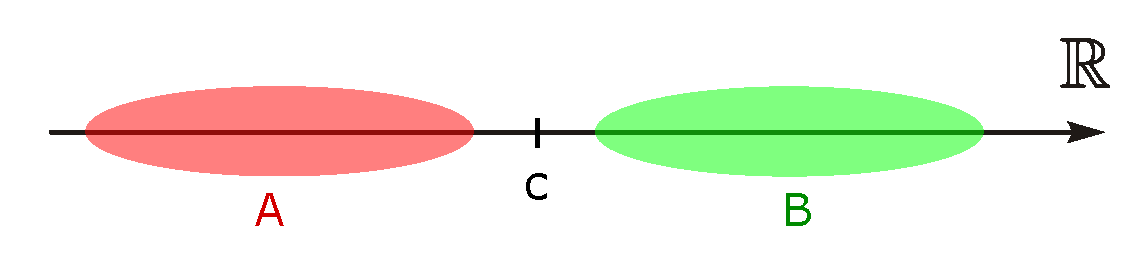
\includegraphics[scale=0.4]{pictR2.pdf}
\end{center}

\end{block}
\pause
Рациональные числа $\mathbb{Q}$ не обладают свойством полноты. Достаточно рассмотреть
$$A=\left\{ q\in\mathbb{Q} \mid q>0,\ q^2<2 \right\},\quad B=\left\{ q\in\mathbb{Q} \mid q>0,\ q^2>2 \right\}.$$

\end{frame}

\begin{frame}{Множества действительной оси}
Мы будем использовать следующие стандартные обозначения для множеств на действительной оси:

\begin{itemize}
\item Отрезок $[a,b]=\{ x\in \mathbb{R} \mid a \le x \le b\}$.
\item Конечный интервал $(a,b)=\{ x\in \mathbb{R} \mid a < x < b\}$.
\item Конечный полуинтервал $(a,b]=\{ x\in \mathbb{R} \mid a < x \le b\}$, или аналогично $[a,b)$.
\item Окрестность точки $x$ --- это произвольный интервал, содержащий точку $x$:
$$U \text{ --- окрестность точки $x$}\quad \iff \quad \exists \alpha,\ \beta\in\mathbb{R}:\quad U=(\alpha,\beta),\ x\in U.$$
\item $\delta$-окрестность точки $x$ --- это интервал $O_\delta(x)=(x-\delta, x+\delta)$.
\item Проколотая $\delta$-окрестность точки $x$ --- это $\delta$-окрестность точки $x$ без самой точки $x$:
$$\dot O_\delta(x)=(x-\delta,x) \cup (x, x+\delta).$$
\end{itemize}
\pause
Иногда при обозначении интервалов уместно использовать символ $+\infty$ и $-\infty$. Например:

$$x\in (-\infty , a] \quad \Leftrightarrow \quad x\le a,$$
$$(-\infty, +\infty) = \mathbb{R}$$
Окрестностями $+\infty$ и $-\infty$ называют интервалы вида $(\alpha,+\infty)$ и $(-\infty,\beta)$ соответственно.
\end{frame}

\begin{frame}{Ограниченные множества}
\begin{block}{Определение}
Множество $A\subset \mathbb{R}$ называется ограниченным сверху (снизу), если существует константа $C$ такая, что $a\le C$ (соответственно $a\ge C$) для всех $a\in A$.
\vskip1em

Такие константы $C$ называются верхними (нижними) гранями множества $A$.
\vskip1em

Множество $A$ называется {\bf ограниченным}, если оно ограниченно как сверху, так и снизу.
\end{block}
\pause
\begin{block}{Примеры}
\begin{enumerate}
\item Интервал $(1,2)$ --- ограниченное множество.
\item Множество $\mathbb{N}$ --- ограниченно  снизу.
\item Множество $\mathbb{Z}$ --- неограниченно.
\end{enumerate}
\end{block}
\end{frame}

\begin{frame}{Ограниченные множества}
\begin{block}{Предложение}
Конечное объединение
$$A=A_1 \cup A_2 \cup \ldots \cup A_n=\bigcup_{j=1}^n A_j$$
ограниченных множеств $A_j$ ($j=1,\ldots,n$) являются ограниченным.
\end{block}
\begin{block}{Доказательство}
Поскольку множества $A_j$ ($j=1,\ldots,n$) является ограниченными, существуют константы $c_j$:
$$|a|\le c_j \quad \forall a\in A_j \quad (j=1,\ldots,n).$$
Определим $c=\max( c_1, c_2, \ldots, c_n )$. Тогда
$$
a\in A=\bigcup_{j=1}^n A_j \quad \Leftrightarrow \quad 
\exists j: a\in A_j \quad \Rightarrow \quad
a\le c_j \quad \Rightarrow \quad
a \le c=\max c_j.
$$
Таким образом, мы доказали, что
$$\exists c\in \mathbb{R}:\qquad  a\in A \quad \Rightarrow \quad |a|\le c.$$
\end{block}
\end{frame}

\begin{frame}{Точная верхняя и нижняя грани}

Для одного ограниченного множества существует много различных верхних и нижних граней. 
Например, для отрезка $[-1,1]$ числа $10, 20, 30, \ldots$, очевидно, являются верхними гранями.
\vskip1em

Возникает естественный вопрос о нахождении наиболее точной оценки для элементов множества.
\pause
\begin{block}{Определение}
Точной верхней гранью (супремумом) ограниченного сверху множества $A$ называют наименьшую возможную верхнею грань множества $A$, пишут:
$$z=\sup A= \sup_{a\in A} a.$$
Таким образом $z=\sup A$ тогда и только тогда, когда выполнены два условия:
\begin{enumerate}
\item число $z$ является верхней гранью множества $A$, то есть $a\le z$ для всех $a\in A$;
\item если $c$ --- верхняя грань множества $A$, то $z\le c$.
\end{enumerate}
\end{block}
\end{frame}

\begin{frame}{Точная верхняя и нижняя грани}

Аналогично определяется точная нижняя грань множества.

\begin{block}{Определение}
Точной нижней гранью (инфинумом) ограниченного снизу множества $A$ называют наибольшую возможную нижнюю грань множества $A$, пишут:
$$z=\inf A= \inf_{a\in A} a.$$
\end{block}
Если множество $A$ неограниченно сверху, то пишут
$$\sup A = +\infty.$$
Если множество $A$ неограниченно снизу, то пишут
$$\inf A = -\infty.$$
Для пустого множества принемают $\inf\emptyset = +\infty$, $\sup\emptyset = -\infty$.

\begin{block}{Упражнение}
Чему равен $\displaystyle \sup_{|x|<1} x$ ? Как это строго обосновать?
\end{block}

\end{frame}

\begin{frame}{Точная верхняя и нижняя грани}

\begin{block}{Предложение}
Если $z=\sup A$, где $A$ --- ограниченное сверху множество, то
$$\forall \varepsilon>0\ \exists a\in A: \quad |z-a| < \varepsilon.$$
\begin{center}
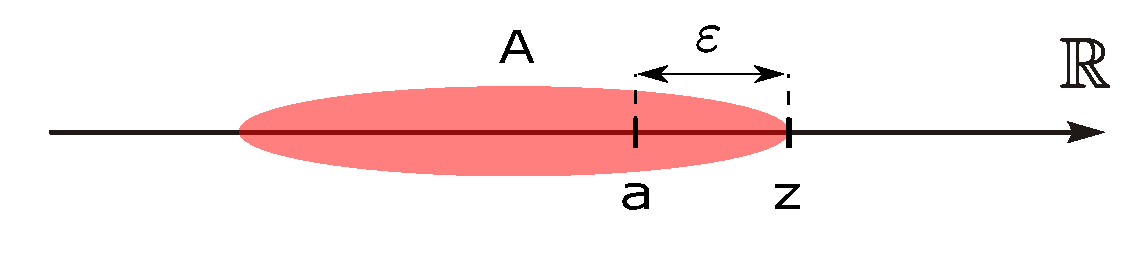
\includegraphics[scale=0.4]{pictR3.pdf}
\end{center}
\end{block}
\vskip-2em
\pause

\begin{block}{Доказательство}
Предположим обратное:
$$\exists \varepsilon_0:\quad \forall a\in A \quad |z-a|\ge \varepsilon_0.$$
Тогда $ z-a \ge \varepsilon_0$, следовательно, $a \le z - \varepsilon_0 < z - \varepsilon_0/2$
для всех $a\in A$.
\vskip1em
\pause

Таким образом мы показали, что число $ z_1=z - \varepsilon_0/2$ является верхней гранью множества $A$, но $z_1<z$, что противоречит определению супремума как наименьшей верхней грани.
\end{block}
\pause

{\bf Упражнение.} Сформулируйте и докажите аналогичное свойство для инфинумов.

\end{frame}

\begin{frame}{Теорема Больцано}

\begin{block}{Теорема Больцано}
Пусть $A\ne\emptyset$ --- ограниченное сверху множество. Тогда
\begin{enumerate}
\item Существует $z\in\mathbb{R}:\ z=\sup A$. 
\item Величина $z=\sup A$ определена однозначно.
\end{enumerate}
\end{block}
\pause

\begin{block}{Доказательство (Существование)}
Рассмотрим множество $B$ всевозможных верхних граней множества $A$. Тогда $B\ne \emptyset$, поскольку множество $A$ ограничено сверху по предположению теоремы, а также
$$\forall a\in A,\ \forall b \in B \quad a \le b$$
по определению верхней грани. Применяя свойство (аксиому) полноты действительных чисел, получаем, что
$$\exists c\in \mathbb{R}: \qquad \forall a\in A,\ \forall b \in B \quad a\le c \le b.$$
Следовательно, $c=\sup A$ как наименьшая из возможных верхних граней.
\end{block}
\end{frame}

\begin{frame}{Теорема Больцано}

\begin{block}{Доказательство (Единственность)}
Предположим обратное. Пусть
$$\exists\ z_1\ne z_2: \quad z_1=\sup A,\  z_2=\sup A.$$
Тогда либо $z_1<z_2$, либо $z_2<z_1$, что сразу противоречит тому, что $\sup A$ --- это наименьшая из возможных верхних граней.
\end{block}

\begin{block}{Замечание}
Утверждение о существовании супремума для любого ограниченного сверху множества можно считать другой формулировкой аксиомы полноты действительных чисел.
\end{block}

\begin{block}{Упражнения}
\begin{enumerate}
\item Докажите свойство полноты действительных чисел, используя теорему Больцано.
\item Сформулируйте и докажите аналогичное утверждение для инфинума.
\end{enumerate}
\end{block}

\end{frame}

\begin{frame}{Функция}
\begin{block}{Отображение}
Отображение (функция, преобразование) $f: A \rightarrow B$ --- это правило, по которому каждому элементу $a$ множества $A$ ставится в соответствие некоторый элемент $b$ множества $B$.
\end{block}


Множество $A$ называют областью определения.

Множество $B$ называют областью значений.

Если элементу $a\in A$ ставится в соответствие элемент $b\in B$, то элемент $b$ называют образом элемента $a$ и пишут $b=f(a)$.

\begin{block}{Пример} 
Отображение $u: \mathbb{Z} \rightarrow \mathbb{N}$ такое, что $\forall n \in \mathbb{Z} \quad u(n)=n^2$.
\end{block}

\begin{block}{Определение. Прообраз}
Прообраз (полный прообраз) элемента $b \in B$ при отображении $f: A \rightarrow B$ --- это множество $f^{-1}(b) \subset A$ всех элементов $a \in A$, которые переходят в $b$ при отображении $f$:
$$f^{-1}(b)  = \left\{ a \in A \mid f(a) = b \right\}.$$
\end{block}

Для заданного примера $u(n)=n^2$:
$$u^{-1}(4) = \{ -2,\ 2 \}, \quad u^{-1}(5) = \emptyset.$$
\end{frame}

\begin{frame}{Сложная функция. Обратная функция}
\begin{block}{Определение. Суперпозиция отображений (сложная функция)}
Пусть задано два отображения  $f: A \rightarrow B$ и  $g: B \rightarrow C$. Тогда суперпозиция отображений  $f$ и $g$ --- это отображение $w: A \rightarrow C$, действующие по правилу:
$$\forall a \in A \quad w(a) = g(f(a))=(g\circ f)(a).$$
\end{block}
\pause
\begin{block}{Определение. Обратное отображение}
Два отображения  $f: A \rightarrow B$ и  $g: B \rightarrow A$ называют взаимно обратными, если
$$\forall a \in A \quad  g(f(a))=a 
\quad\text{ и }\quad 
\forall b \in B \quad  f(g(b))=b.$$
\end{block}
\pause
\begin{block}{Примеры обратных функций}
\begin{itemize}
\item $y=x^2$ и $x=\sqrt{y}$ для $x\ge 0$;
\item $y=1/x$ и $x=1/y$ для $x\ne 0$;
\item $y=\sin(x)$ и $x=\arcsin(y)$ для $x\in [-\pi/2, \pi/2 ]$.
\end{itemize}
\end{block}
\end{frame}

\begin{frame}{Биективное отображение}
\begin{block}{Определение. Взаимно однозначное соответствие (биекция)}
Отображение  $f: A \rightarrow B$ называется биективным, если для каждого элемента $b\in B$ существует единственный элемент $a\in A$ такой, что $f(a)=b$.
\end{block}

\begin{block}{Предложение. Условия существования обратной функции}
Для отображения $f$ существует обратное отображение тогда и только тогда, когда отображение $f$ биективно.
\end{block}
Доказательство проведите самостоятельно.

\begin{block}{Препятствия для существования обратного отображения}

\begin{center}
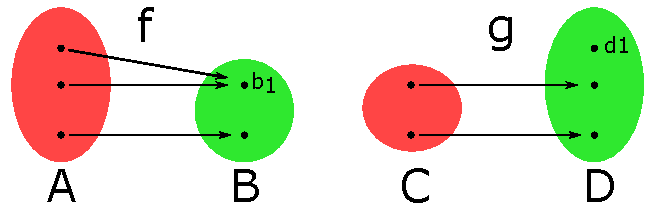
\includegraphics[scale=0.7]{set1.pdf}
\end{center}
Отображение $f$ --- не инъективно , а отображение $g$ --- не сюръективно.
\end{block}
\end{frame}

\begin{frame}{График функции}
\begin{block}{Определение. График функции}
Графиком функции  $f: A \rightarrow B$ называется множество всех пар $(a,b)$, где $a\in A$ и $b=f(a)$.
\end{block}
Для числовых функций графики удобно изображать на плоскости $(x,y)$.
\begin{block}{Пример}
График функции $y=x^2$ и обратной функции $\sqrt{x}$:

\begin{center}
\only<1>{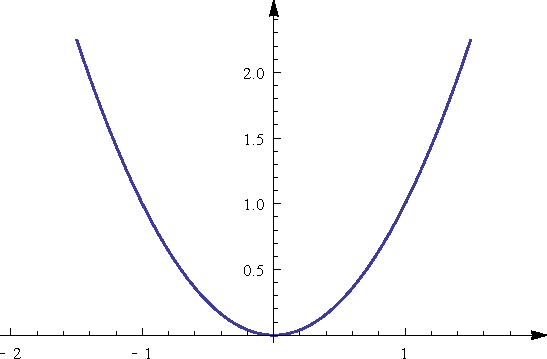
\includegraphics[scale=0.6]{x2p1.pdf}}
\only<2>{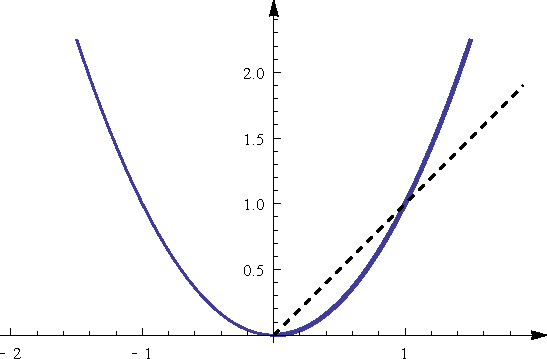
\includegraphics[scale=0.6]{x2p2.pdf}}
\only<3>{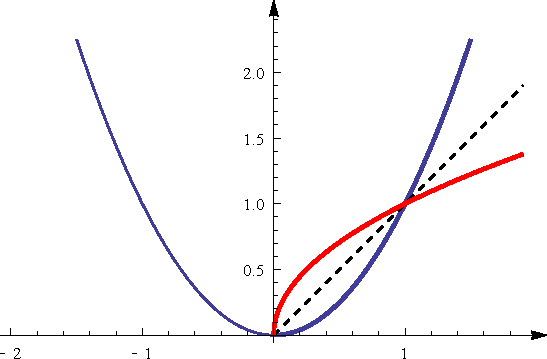
\includegraphics[scale=0.6]{x2p3.pdf}}
\end{center}
График обратной функции получается при отражении графика функции относительно прямой $y=x$.
\end{block}
\end{frame}

\begin{frame}{Последовательности}

\begin{block}{Определение. Последовательность}
Числовой последовательностью называют произвольную функция $a$ из $\mathbb{N}$ в $\mathbb{R}$.
\end{block}
Часто вместо $a(n)$  пишут $a_n$.
\pause
\vskip1em
Последовательность может быть задана в виде явной формулы для общего члена последовательности $a_n=\ldots$ 

\vskip1em
Возможно также задание с помощью неявной (например, рекурсивной) формулы или просто при помощи некоторого корректного описания.
\begin{block}{Примеры}
\begin{itemize}
\item $a_n=1/n$;
\item $a_0=3$, $a_1=3.1$, $a_2=3.14$ и так далее, где $a_n$ --- десятичные приближения к числу $\pi$;
\item $F_1=1$, $F_2=1$, $F_{n+2}=F_n + F_{n+1}$ --- числа Фибоначчи.
\end{itemize}
\end{block}

\end{frame}

\begin{frame}{Предел последовательности}

\begin{block}{Определение. Предел последовательности}
Число $a$ называют {\bf пределом последовательности} $a_n$, если для любого наперед заданного числа $\varepsilon>0$ все члены последовательности $a_n$, начиная с некоторого номера $N$, лежат в $\varepsilon$-окрестности точки $a$:
$$\forall \varepsilon>0\ \exists N=N(\varepsilon):\ \forall n\ge N \quad |a_n-a|<\varepsilon.$$
Записывают это так: $\lim\limits_{n\to +\infty} a_n = a$ или $a_n\to a$.
\end{block}

\begin{center}
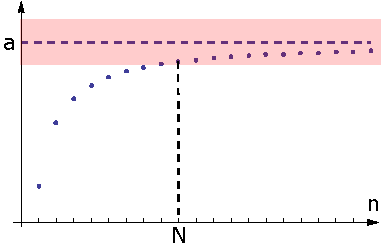
\includegraphics[scale=1]{lim.pdf}
\end{center}

\end{frame}


\begin{frame}{Предел последовательности}
\begin{block}{Определение}
Аналогично вводятся понятия бесконечного предела. Разделяют три случая:
\begin{enumerate}
\item $a_n\to +\infty \qquad \Leftrightarrow \qquad 
\forall A>0\ \exists N=N(A):\ \forall n\ge N \quad a_n > A;$
\item  $a_n\to -\infty \qquad \Leftrightarrow \qquad 
\forall A>0\ \exists N=N(A):\ \forall n\ge N \quad a_n < -A;$
\item  $a_n\to \infty \phantom{-} \qquad \Leftrightarrow \qquad 
\forall A>0\ \exists N=N(A):\ \forall n\ge N \quad |a_n| > A.$
\end{enumerate}
\end{block}

\begin{block}{Определение}
\begin{itemize}
\item Последовательность $a_n$ называется {\bf сходящейся}, если у нее существует конечный предел.
\item Последовательность $a_n$ называется {\bf бесконечно малой}, если $a_n\to 0$.
\item Последовательность $a_n$ называется {\bf бесконечно большой}, если $a_n\to \infty$.
\end{itemize}
\end{block}

\begin{block}{Упражнения}
Приведите примеры последовательностей, отвечающих данным определениям.
\end{block}

\end{frame}

\begin{frame}{Предел последовательности}
\begin{block}{Примеры}
\begin{enumerate}
\item Последовательность $a_n=1/n$:
$$\lim_{n\to+\infty}\frac{1}{n}=0.$$
Действительно, для любого $\varepsilon>0$ возьмем $N$, равное целой части $\varepsilon^{-1}+1$. Тогда
$$n\ge N \quad\Rightarrow\quad n> \frac{1}{\varepsilon} \quad\Rightarrow\quad |a_n|<\varepsilon,$$
что и требовалось показать.
\item Последовательность $b_n=n^2$:
$$\lim_{n\to+\infty}n^2=+\infty.$$
Доказательство:
$$\forall A>0\ \exists N=[\sqrt{A}+1]: \quad n\ge N\ \Rightarrow\ b_n=n^2\ge N^2>A.$$
\item Последовательность $c_n=(-1)^n$:
$$\nexists\  \lim_{n\to+\infty}c_n.$$
\end{enumerate}
\end{block}

\end{frame}


\begin{frame}{Единственность предела}
\begin{block}{Теорема}
Предел сходящейся последовательности определен однозначно.
\end{block}
\begin{block}{Доказательство}
Предположим обратное. Пусть $a_n$ --- сходящаяся последовательность, числа $s_1$ и $s_2\ne s_1$  --- ее пределы. Тогда возьмем $\varepsilon=|s_2-s_1|/2$. По определению предела получаем:
$$a_n\to s_1 \quad \Rightarrow \quad \exists N_1:\ \forall n\ge N_1\quad |a_n-s_1|<\varepsilon,$$
$$a_n\to s_2 \quad \Rightarrow \quad \exists N_2:\ \forall n\ge N_2\quad |a_n-s_2|<\varepsilon.$$
Если $N=\max(N_1,N_2)$, то
$$|s_1 - s_2|=|(s_1 - a_N) + (a_N - s_2)|\le |a_N - s_1| + |a_N - s_2| < 2\varepsilon = |s_2 - s_1|.$$
Получили противоречие вида $|s_1-s_2|<|s_1 - s_2|$.
\end{block}

\begin{block}{Замечание}
Предел вида $a_n\to \pm\infty$ также определен однозначно. Например, последовательность не может одновременно иметь конечный предел и стремиться к $+\infty$.
\end{block}

\end{frame}

\begin{frame}{Арифметические свойства предела}
\begin{block}{Теорема}
Пусть $a_n\to a$ и $b_n\to b$ --- сходящиеся последовательности. Тогда
\begin{enumerate}
\item $\displaystyle \lim_{n\to+\infty} (c_1 a_n + c_2 b_n) = c_1 a+ c_2 b$;\quad (Свойство линейности)
\item $\displaystyle \lim_{n\to+\infty} a_n b_n = a b$;
\item Если $b\ne 0$, то $\displaystyle \lim_{n\to+\infty} a_n/b_n = a / b$.
\end{enumerate}
\end{block}
\vskip-1em
\begin{block}{Доказательство}
Поскольку $a_n\to a$ и $b_n\to b$ получаем, что
$$\forall \varepsilon'>0\ \exists N_1:\ \forall n\ge N_1 \quad |a_n-a|<\varepsilon',$$
$$\forall \varepsilon'>0\ \exists N_2:\ \forall n\ge N_2 \quad |b_n-b|<\varepsilon'.$$
Тогда при $n>N=\max( N_1, N_2)$
$$|(c_1 a_n + c_2 b_n) - (c_1 a+ c_2 b)|\le |c_1| |a_n -a| + |c_2| |b_n-b|< (|c_1|+|c_2|)\varepsilon'.$$
Следовательно, выбирая $\varepsilon'=\varepsilon/(|c_1|+|c_2|)$, получим
$$\forall \varepsilon>0\ \exists N:\ \forall n\ge N \quad |(c_1 a_n + c_2 b_n)-(c_1 a+ c_2 b)|<\varepsilon,$$
что и требовалось доказать.
\end{block}
\end{frame}

\begin{frame}{Арифметические свойства предела. Неопределенности}
\begin{block}{Определение}
Говорят, что для последовательности $u_n$ имеет место неопределенность вида
\begin{enumerate}
\item ``$\infty - \infty$'' если $u_n= a_n - b_n$, где $a_n\to \infty$ и $b_n \to \infty$;
\item ``$\infty \times 0$'' если $u_n= a_n b_n$, где $a_n\to \infty$ и $b_n \to 0$;
\item ``$\displaystyle \frac{0}{0}$'' если $\displaystyle u_n= \frac{a_n}{b_n}$, где $a_n\to 0$ и $b_n \to 0$;
\item ``$\displaystyle \frac{\infty}{\infty}$'' если $\displaystyle u_n= \frac{a_n}{b_n}$, где $a_n\to \infty$ и $b_n \to \infty$.
\end{enumerate}
\end{block}
\begin{block}{Упражнение}
Приведите примеры для каждого случая такие, что 
\begin{enumerate}
\item $u_n$ --- сходится;
\item $u_n$ является бесконечно малой или бесконечно большой;
\item предел $u_n$ не существует.
\end{enumerate}
\end{block}
\end{frame}

\begin{frame}{Арифметические свойства предела. Пример}

Рассмотрим последовательность
$$r_n=\frac{2n^2+2n+7}{n^2+1}.$$
Это неопределенность вида ``$\frac{\infty}{\infty}$''. Разделим числитель и знаменатель на $n^2$:
$$r_n=\frac{2+2/n+7/n^2}{1+1/n^2}.$$
Рассмотрим последовательности, отвечающие числителю и знаменателю соответственно:
$$a_n=2+2/n+7/n^2,\quad b_n=1+1/n^2.$$
Учитывая свойство линейности предела и то, что $1/n$ и $1/n^2$ стремятся к $0$, получаем, что
$$a_n\to 2,\quad b_n\to 1.$$
Поскольку предел последовательности $b_n$ (знаменателя для $r_n$) не равен $0$, получаем, что
$$\lim_{n\to+\infty} r_n = \lim_{n\to+\infty} \frac{a_n}{b_n} = \frac{\lim\limits_{n\to+\infty} a_n}{\lim\limits_{n\to+\infty} b_n}=\frac{2}{1}=2.$$
Таким образом,
$$\lim_{n\to\infty} \frac{2n^2+2n+7}{n^2+1} = 2.$$
\end{frame}


\begin{frame}{Переход к пределу в неравенствах}
\begin{block}{Теорема}
Пусть $a_n\to a$ и $b_n \to b$  --- сходящиеся последовательности, и 
$$a_n\le b_n,$$
для всех $n$, начиная с некоторого номера $M$.
Тогда
$$a\le b$$
\end{block}
\vskip-1em
\begin{block}{Доказательство}
Предположим обратное. Пусть $a>b$. Тогда, выбирая $\varepsilon=(a-b)/2$, получаем, что
$$\exists N: \ \forall n\ge N\qquad |a_n - a|<\varepsilon, \quad |b_n - b|<\varepsilon.$$
Следовательно, если $n>N$, то
$$a_n > a - \varepsilon = a - \frac{a-b}{2} = \frac{a+b}{2},$$
$$b_n < b + \varepsilon = b + \frac{a-b}{2} = \frac{a+b}{2}.$$
Получили, что $a_n>b_n$ при $n>N$. Это противоречит тому, что $a_n \le b_n$, при $n>M$.
\end{block}

\end{frame}

\begin{frame}{Лемма ``о двух милиционерах''}
\begin{block}{Лемма}
Пусть $a_n$  и $c_n$ --- сходящиеся последовательности:
$$\lim_{n\to+\infty} a_n = \lim_{n\to+\infty} c_n = L,$$
и справедливо неравенство:
$$a_n\le b_n \le c_n.$$
Тогда последовательность $b_n$ также является сходящейся и
$$\lim_{n\to\infty} b_n = L.$$
\end{block}
\vskip-1em
\begin{block}{Пример}
Рассмотрим последовательность
$$s_n=\frac{\sin(n)}{n}.$$
Последовательность $s_n\to 0$, поскольку справедливо неравенство:
$$-\frac{1}{n} \le \frac{\sin(n)}{n} \le \frac{1}{n}.$$
\end{block}
\end{frame}

\begin{frame}{Сравнение бесконечно больших последовательностей}
\begin{block}{Предложение}
Пусть $a_n\to + \infty$. Если $b_n \ge a_n$, то $\lim b_n =+\infty$.
\end{block}

\begin{block}{Пример}
Рассмотрим последовательность
$$u_n=\frac{a^n}{n},\quad a>1.$$
Покажем, что величина $a^n$ растет очень быстро. Неравенство
$$a^n \ge 1 + n (a-1) + \frac{n(n-1)}{2} (a-1)^2$$ 
можно доказать по индукции ({\bf докажите!}). Следовательно,
$$\frac{a^n}{n}\ge \frac{1}{n}+a-1+\frac{1}{2}(n-1)(a-1)^2\ge 
\frac{(a-1)^2}{2}(n-1)  \to +\infty$$
Таким образом,
$$\lim_{n\to+\infty}\frac{a^n}{n} = +\infty \qquad (a>1).$$
\end{block}

\end{frame}


\begin{frame}{Монотонные последовательности}
\begin{block}{Определение. Монотонные последовательности}
Числовая последовательность называется возрастающей (неубывающей), если $a_{n+1} > a_n$ (соответственно, $a_{n+1} \ge a_n$) для всех $n\in\mathbb{N}$.
\vskip0.5em
Числовая последовательность называется убывающей (невозрастающей), если $a_{n+1} < a_n$ (соответственно, $a_{n+1} \le a_n$) для всех $n\in\mathbb{N}$.
\vskip0.5em
Такие последовательности называют \bf монотонными.
\end{block}
\pause

\begin{block}{Определение. Ограниченные последовательности}
Числовая последовательность называется ограниченной сверху (снизу), если $\exists c\in \mathbb{R}$ такая, что $a_{n}< c$ (соответственно, $a_n >c$) для всех $n\in\mathbb{N}$.
\vskip0.5em
Числовая последовательность называется {\bf ограниченной}, если она ограничена как сверху, так и снизу, то есть $$\exists c\in \mathbb{R}:\quad |a_n|<c\quad \forall n\in\mathbb{N}.$$
\end{block}
\pause

\begin{block}{Упражнение}
Докажите, что любая сходящаяся последовательность ограничена.
\end{block}

\end{frame}

\begin{frame}{Теорема о пределе монотонной последовательности}

\begin{block}{Теорема Вейерштрасса}
Монотонная ограниченная последовательность сходится.
\end{block}
\begin{block}{Доказательство}
Пусть $a_n$ --- монотонная ограниченная последовательность. Для определенности предположим, что $a_n$ не убывает.
Поскольку последовательность $a_n$ ограничена сверху, то (т. Больцано) существует
$$z=\sup_{n\ge1} a_n = \sup A < +\infty,$$
где $A = \left\{ a_n,\ n\in\mathbb{N} \right\}$ --- множество всех значений последовательности $a_n$.
\vskip1em
По свойству супремума
$$\forall \varepsilon>0\ \exists a\in A:\quad |z-a| < \varepsilon.$$
Поскольку
$$a\in A \quad \Leftrightarrow \quad \exists N:\ a=a_N
\qquad \text{и} \qquad
a_n \ge a_N, \quad \text{при $n\ge N$},$$
получаем, что
$$|z - a_n| = z - a_n \le z - a_N < \varepsilon.$$
Таким образом,
$$\lim_{n\to +\infty} a_n = \sup_{n\ge1} a_n.$$
\end{block}
\end{frame}

\begin{frame}{Пример вычисления предела}
\begin{block}{Пример}
Рассмотрим последовательность $\displaystyle a_n=\frac{2^n}{n!}$.
Проверим на монотонность:
$$\frac{a_{n+1}}{a_n}=\frac{ 2^{n+1}}{(n+1)!}\frac{n!}{2^n}=\frac{2}{n+1}\le1
\quad \Rightarrow \quad
a_{n+1}\le a_n.$$
Последовательность убывает (при $n>1$) и ограничена снизу ($a_n\ge 0$), следовательно, она сходится:
$$\lim_{n\to+\infty}a_n=x.$$
Перейдем в равенстве
$$a_{n+1} = a_n \frac{2}{n+1}$$
к пределу при $n\to+\infty$:
$$\lim_{n\to+\infty} a_{n+1} = \lim_{n\to+\infty}\Big(  a_n \frac{2}{n+1} \Big)
\quad \Rightarrow \quad
x = \lim_{n\to+\infty}a_n \cdot \lim_{n\to+\infty}\frac{2}{n+1} = x \cdot 0=0.$$
Получили, что $2^n/n! \to 0$.
\end{block}
\end{frame}

\begin{frame}{Пример вычисления предела}
\begin{block}{Пример}
Рассмотрим последовательность
$$\sqrt{2},\ \sqrt{2+\sqrt{2}},\ \sqrt{2+\sqrt{2+\sqrt{2}}},\ldots$$
или
$$a_1=\sqrt{2},\quad a_{n+1}=\sqrt{2+a_n}.$$
Последовательность ограничена:
$$0\le a_n \le 2,$$
и монотонно возрастает:
$$a_{n+1} - a_n = \sqrt{2+a_n} - a_n = \frac{2+a_n-a_n^2}{\sqrt{2+a_n} + a_n }=
\frac{(2-a_n)(1+a_n)}{\sqrt{2+a_n} + a_n }\ge 0.
$$
Следовательно, последовательность является сходящейся $a_n\to z$. Переходя к пределу в равенстве $ a_{n+1}=\sqrt{2+a_n}$, получаем, что
$$z=\sqrt{2+z} \quad \Rightarrow \quad z^2-z-2=0,\ z\ge0 \quad\Rightarrow\quad z=2.$$

\end{block}
\end{frame}

\begin{frame}{Бином Ньютона. Биномиальные коэффициенты}
\begin{block}{Бином Ньютона}
$$(a+b)^n = a^n + n a^{n-1} b + \cdots + n a b^{n-1} + b^n = 
\sum_{k=0}^n C_n^k a^{n-k} b^k,$$
где $C_n^k$ --- число сочетаний из $n$ по $k$ (биномиальный коэффициент):
$$C_n^k = \binom{n}{k} = \frac{n!}{k! (n-k)!}.$$ 
\end{block}
\begin{block}{Свойства биномиальных коэффициентов}
\begin{enumerate}
\item Симметрия:
$$C_n^k = C_n^{n-k}.$$
\item Разложение для $2^n$:
$$2^n = (1+1)^n = C_n^0+ \cdots + C_n^n.$$
\item Треугольник Паскаля:
$$C_n^k = C_{n-1}^{k-1} + C_{n-1}^k.$$
\end{enumerate}
\end{block}
\end{frame}

\begin{frame}{Число $e$}
\begin{block}{Определение}
Числом $e$ называют предел последовательности:
$$a_n=\left( 1 + \frac{1}{n} \right)^{n}.\quad (n\to+\infty)$$
\end{block}
\vskip-1em
\pause
\begin{block}{Предложение (корректность определения)}
Последовательность $a_n$ является сходящейся.
\end{block}
\pause
\begin{block}{Упражнения}
\begin{enumerate}
\item Докажите, что последовательность $a_n$ возрастает (используйте бином Ньютона).
\item Докажите, что последовательность $a_n$ ограничена. Указание:
$$a_n \le 2+\sum_{k=2}^n \frac{1}{k!} \le 2 + \sum_{k=0}^n\frac{1}{2^k} \le 3.$$
\item Докажите, что последовательность $(1+1/n)^{n+1}$ убывает и
$$\left(1+\frac{1}{n}\right)^n<e<\left(1+\frac{1}{n}\right)^{n+1}.$$
\end{enumerate}
\end{block}
\end{frame}


\begin{frame}{Верхний и нижний предел}

Пусть $a_n$ --- ограниченная последовательность. Рассмотрим
$$i_n = \inf_{k\ge n} a_k,\qquad s_n = \sup_{k\ge n} a_k.$$
Последовательности $i_n$ и $s_n$ монотонны и ограниченны, следовательно, они являются сходящимися.
\begin{block}{Определение}
Верхним пределом последовательности $a_n$ называют
$$\varlimsup_{n\to+\infty}  a_n = \lim_{n\to+\infty}  \sup_{k\ge n} a_k.$$
Нижним пределом последовательности $a_n$ называют
$$\varliminf_{n\to+\infty}  a_n = \lim_{n\to+\infty}  \inf_{k\ge n} a_k.$$
\end{block}
\vskip-1em
\pause
\begin{block}{Упражнение}
\begin{enumerate}
\item Докажите, что нижний предел нестрого меньше верхнего предела.
\item Докажите, что последовательность сходится тогда и только тогда, когда ее верхний и нижний пределы конечны и совпадают.
\end{enumerate}
\end{block}

\end{frame}

\begin{frame}{Критерий Коши}
\begin{block}{Определение}
Последовательность $x_n$ называют {\bf фундаментальной} (последовательностью Коши), если 
$$\forall \varepsilon>0\ \exists N:\ \forall n\ge N\ \text{и}\ m\ge N \quad |x_n - x_m|<\varepsilon.$$
\end{block}
\vskip-1em
\pause
\begin{block}{Теорема. Критерий сходимости последовательностей}
Последовательность $a_n$ является сходящейся тогда и только тогда, когда она является последовательностью Коши.
\end{block}
\pause
\begin{block}{Упражнения}
\begin{enumerate}
\item Докажите, что сходящаяся последовательность фундаментальна.
\item Докажите, что фундаментальная последовательность ограничена.
\item Докажите, что верхний и нижний предел фундаментальной последовательности совпадают. Указание:
$$|x_n - x_m| < \varepsilon \quad \Rightarrow \quad 
|\sup_{k\ge n} x_k - \inf_{k\ge n} x_k| < \varepsilon
$$
\end{enumerate}
\end{block}
\end{frame}

\begin{frame}{Подпоследовательность}
\begin{block}{Определение (Подпоследовательность)}
Последовательность $b_k$ называют {\bf подпоследовательностью} последовательности $a_n$, если
$$b_k = a_{n_k},\ (k=1,2,\ldots),$$
где $n_k$ возрастающая последовательность натуральных чисел:
$$n_1<n_2<\ldots<n_k<n_{k+1}<\ldots$$
\end{block}
\vskip-1em
\begin{block}{Определение (Частичный предел)}
Частичными пределами последовательности $a_n$ называют пределы ее подпоследовательностей.
\end{block}
\begin{block}{Свойства}
\begin{enumerate}
\item В любой окрестности частичного предела лежит бесконечно много членов последовательности. Верно и обратное: если в любой окрестности точки лежит бесконечно много членов последовательности, то эта точка --- частичный предел последовательности.

\item Сходящаяся последовательность имеет единственный частичный предел, который равен ее пределу.
\end{enumerate}
\end{block}
\end{frame}

\begin{frame}[t]{Подпоследовательность}

\begin{block}{Теорема}
Верхний (нижний) предел последовательности являются супремумом (инфинумом) множества всех частичных пределов последовательности.
\end{block}
\vskip-1em
\begin{block}{Доказательство \onslide+<2>{(Продолжение)}}
\begin{overprint}
\onslide<1>
Для начала докажем, что для заданной последовательности существует подпоследовательность сходящаяся к ее верхнему пределу, то есть верхний предел является одним из частичных пределов последовательности. Пусть
$$a=\varlimsup_{n\to+\infty}a_n 
\quad \Leftrightarrow\quad
\forall \varepsilon'>0\ \exists N:\ \forall n\ge N \quad |a -  \sup_{k\ge n} a_k|<\varepsilon'$$
По свойству супремума:
$$
s_n=\sup_{k\ge n} a_k 
\quad \Leftrightarrow\quad
\forall \varepsilon'\ \exists m_n\ge n:\quad 
|s_n - a_{m_n}| < \varepsilon'.$$
Следовательно, взяв $\varepsilon = \varepsilon'/2$ получаем, что
$$|a-a_{m_n}|\le |a -s_n|+|s_n - a_{m_n}|<2\varepsilon'=\varepsilon \qquad (\forall n\ge N)$$

\onslide<2>
Мы доказали, что верхний предел является одним из частичных пределов последовательности. Остается доказать, что любой другой частичный предел не превосходит верхнего предела. 
\vskip0.5em
Пусть $L$ --- частичный предел последовательности $a_n$: $a_{r_n} \to L \quad (n\to+\infty)$.
Последовательность $s_{r_n}=\sup_{k\ge r_n} a_k$ является подпоследовательностью сходящейся последовательности $s_n=\sup_{k\ge n} a_k$, следовательно,
$$\sup_{k\ge r_n} a_k \to a=\varlimsup_{n\to+\infty} a_n \quad  (n\to+\infty).$$
Переходя к пределу (при $n\to +\infty$) в неравенстве
$$a_{r_n}\le \sup_{k\ge r_n} a_k \quad \Rightarrow\quad  L\le a,$$
получаем необходимую оценку.
\end{overprint}
\end{block}
\end{frame}

\begin{frame}{Свойства частичных пределов}
\begin{block}{Свойства}
\begin{enumerate}
\item Все частичные пределы последовательности лежат между верхним и нижним пределом последовательности.
\item Если для ограниченной последовательности верхний и нижний предел совпадают, то последовательность сходится.
\item Любая ограниченная последовательность имеет сходящуюся подпоследовательность, то есть непустое множество частичных пределов. (Лемма Больцано-Вейерштрасса)
\end{enumerate}
\end{block}
\begin{center}
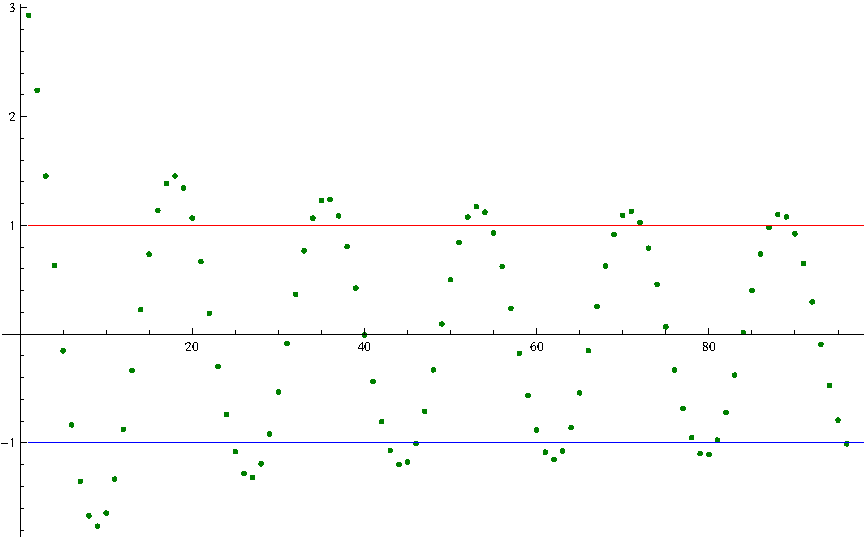
\includegraphics[scale=0.5]{limsup.pdf}
\end{center}
\end{frame}

\end{document}
